\section{Vergleich verschiedener Machine Learning Algorithmen}
Wir nehmenen die Daten von MNIST
\subsection{KNN (Dirk)}

\subsection{Support Vector Machine (Alex)}
Die \textit{Support Vector Machine} (SVM) ist ein Algorithmus zur Klassifizierung von Daten in verschiedene Klassen.
Sie wurde in den 1990er Jahren innerhalb der Informatiker-Community entwickelt und gewinnt seitdem immer weiter an Popularität.
SVMs können in vielen verschiedenen Szenarien eingesetzt werden und werden zu den besten Klassifizierern gezählt.
Bevor die SVM entwickelt wurde gab es verschiedene Vorgängertechnologien aus denen am Ende die heutige \textit{Support Vector Machine} hervorgegangen ist. 
Diese Algorithmen sind einmal der \textit{Maximal Margin Classifier} und der \textit{Support Vector Classifier}, 
der eine Weiterentwicklung des Zuvorgenannten darstellt.
Die \textit{Support Vector Machine} ist wiederum eine Erweiterung des \textit{Support Vector Classifier}.
Alle diese Klassifizierer werden meist lose unter dem Begriff \textit{Support Vector Machine} zusammengefasst,
müssen jedoch klar unterschieden werden.\cite[S. 337]{james_2013}

Die Terminologie im Bereich der \textit{Support Vector Machine} ist nicht ganz klar und kann sich in verschiedenen Veröffentlichungen unterscheiden.
Eine andere Differenzierung der Vorgängertechnologien ist die Einteilung in Lineare Klassifizierer und Nichtlineare Klassifizierer.
Auch zu erwähnen ist der Lagrangische \textit{Support Vector Machine} Algorithmus (LSVM), mit dem iterativ SVMs trainiert werden können.\cite[S. 207]{suthaharan_2015}
In dieser Arbeit verwenden wir die zuvor genannte Einteilung in \textit{Maximal Margin Classifier}, \textit{Support Vector Classifier}
und \textit{Support Vector Machine}. An ihr lässt sich die kontinuierliche Weiterentwicklung der Algorithmen am besten verfolgen und am übersichtlichsten darstellen.
Außerdem wird die Chronologie der hinzugekommenen Konzepte deutlicher.

Beginnen wir mit der einfachsten Form dieser Klassifizierer, dem \textit{Maximal Margin Classifier}. 
Dieser wird durch eine sogenannte \textit{Hyperplane} definiert. In einem $p$-dimensionalen Raum ist eine \textit{Hyperplane}
ein flacher affiner Subraum der Dimension $p - 1$. 
Bei zwei Dimensionen wäre eine \textit{Hyperplane} ein flacher $1$-dimensionaler Subraum oder in anderen Worten eine Gerade.
In einem $3$-dimensionalen Raum ist die \textit{Hyperplane} demnach eine Ebene.
\textit{Hyperplanes} in höherdimensionalen Räumen sind schwer für den Menschen vorstellbar, folgen jedoch ebenfalls der Definition.  
Die mathematische Definition einer \textit{Hyperplane} im $2$-dimensionalen Raum lautet:
\[\beta_0 + \beta_1X_1 + \beta_2X_2 = 0\]
mit den Parametern $\beta_0$, $\beta_1$ und $\beta_2$. 
Es lässt sich erkennen, dass die Definition mit der einer Geraden übereinstimmt und damit unserer oben beschriebenen
Definition einer \textit{Hyperplane} folgt.
In einem $p$-dimensionalen Raum wird die Gleichung einer \textit{Hyperplane} wie folgt erweitert:
\[\beta_0 + \beta_1X_1 + \beta_2X_2  + \dots + \beta_pX_p= 0\]
Eine \textit{Hyperplane} teilt den $p$-dimensionalen Raum in zwei Hälften.
Erfüllt ein Punkt $X = (X_1, X_2, \dots, X_p)$ des $p$-dimensionalen Raumes nicht die obige Gleichung,
liegt er entweder auf der einen Seite
\[\beta_0 + \beta_1X_1 + \beta_2X_2  + \dots + \beta_pX_p> 0\]
oder auf der anderen Seite der \textit{Hyperplane}
\[\beta_0 + \beta_1X_1 + \beta_2X_2  + \dots + \beta_pX_p< 0\]
Abbildung \ref{fig:Hyperplane} zeigt beispielhaft eine solche \textit{Hyperplane}, die durch die Gleichung $1 + 6X_1 + 4X_2 = 0$ definiert ist.
Sie trennt den Raum in einen blauen Bereich, wo alle Punkte $1 + 6X_1 + 4X_2 > 0$ erfüllen und eine rote Seite, auf der für alle Punkte $1 + 6X_1 + 4X_2 < 0$ gilt.
\cite[S. 338]{james_2013}
\begin{figure}[H]
	\centering
	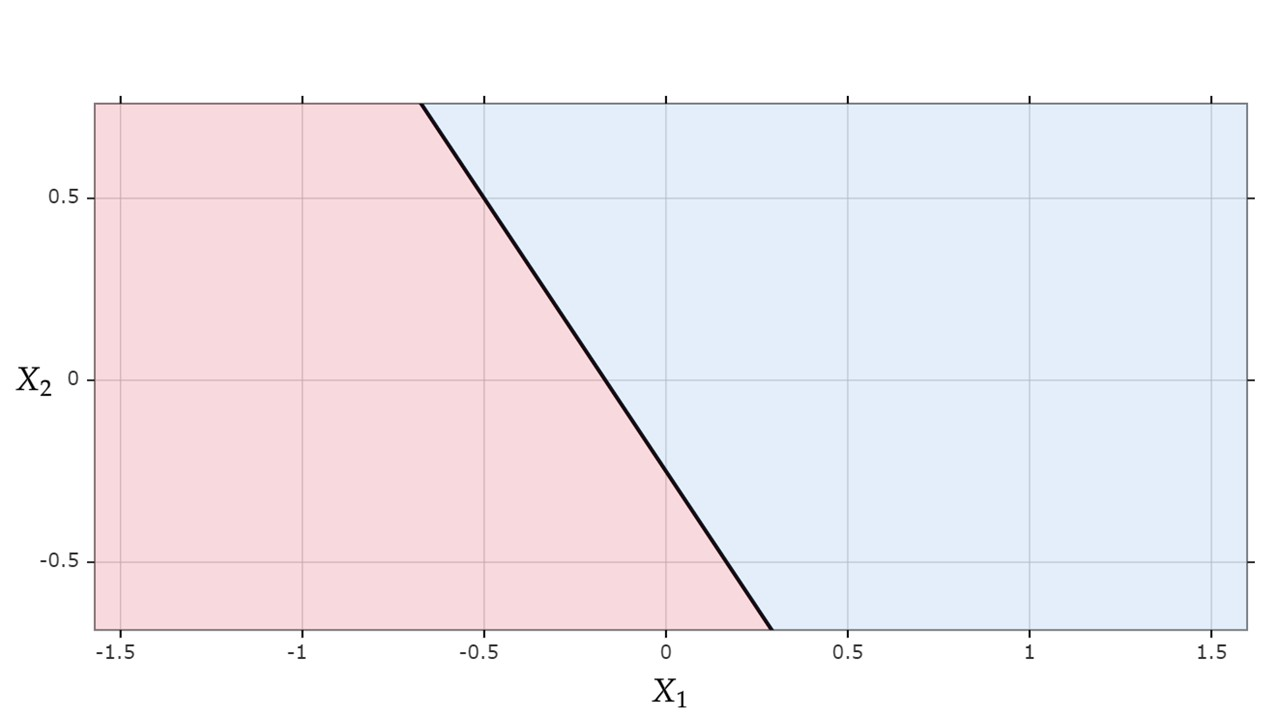
\includegraphics[width=\imgMed]{images/theory/hyperplane.jpg}
	\caption{Beispiel für eine \textit{Hyperplane}} 
	\label{fig:Hyperplane}
\end{figure}
Wir haben nun eine Matrix der Trainingsdaten $\mathbf{X}$ der Form $n \times p$, 
die aus $n$ Trainingsobjekten innerhalb eines $p$-dimensionalen Raumes besteht.
\[x_1 = \left(\begin{array}{c} x_{11} \\ \vdots \\ x_{1p} \end{array}\right) 
  , \dots, 
  x_n = \left(\begin{array}{c} x_{n1} \\ \vdots \\ x_{np} \end{array}\right) \]
Diese Trainingsobjekte sind definiert als Vektoren der Länge $p$, die die einzelnen beobachteten \textit{Features} 
$x^* = (x_1^* \dots x_p^*)^T$ enthalten und werden jeweils einer von zwei Klassen zugeordnet $y_1,\dots,y_n \in \{-1,1\}$.
Wenn die \textit{Hyperplane} die Trainingsobjekte perfekt anhand ihrer Label trennt,
dann spricht man von einer \textit{separierenden Hyperplane}. 
Alle Objekte aus der einen Klassen fallen auf die linke Seite der \textit{Hyperplane}.
Während die Trainigsobjekte mit dem anderen Label auf der rechten Seite der \textit{Hyperplane} liegen.
Eine \textit{separierende Hyperplane} lässt sich mathematisch definieren durch folgende zwei Gleichungen:
\[\beta_0 + \beta_1X_1 + \beta_2X_2  + \dots + \beta_pX_p> 0 \text{ if } y_i = 1\]
\[\beta_0 + \beta_1X_1 + \beta_2X_2  + \dots + \beta_pX_p< 0 \text{ if } y_i = -1\]
für alle $i = 1 , \dots, n$.
Diese \textit{separierende Hyperplane} kann nun als Klassifizierer eingesetzt werden. 
Um ein unbekanntes Testobjekt nun zu klassifizieren, muss nur geschaut werden auf welcher Seite der \textit{Hyperplane} das Objekt liegt.
Liegt das Testobjekt auf der positiven Seite der \textit{Hyperplane} wird ihm das Label $1$ zugewiesen.
Wenn es auf der negativen Seite liegt, wird das Testobjekt der Klasse $-1$ zugeordnet.
Je weiter entfernt das Testobjekt von der \textit{separierenden Hyperplane} liegt, desto sicherer können wir uns sein,
dass die Klassenzuweisung korrekt ist. Je kleiner der Abstand zur \textit{Hyperplane} wird, desto unsicherer ist,
ob das Testobjekt der richtigen Klasse zugeordnet worden ist. 
Der Abstand der einzelnen Testobjekte zur \textit{separierenden Hyperplane} zeigt uns mit welcher Gewissheit das SVM
die richtige Klassifizierung getroffen hat.\cite[S. 339 - 141]{james_2013}

Beim \textit{Maximal Margin Classifier} wird die oben genannte Methode der \textit{separierenden Hyperplane} eingesetzt,
um Daten klassifizieren zu können. Wenn die Daten durch eine \textit{separierende Hyperplane} getrennt werden können,
gibt es unendlich viele Möglichkeiten, wie diese liegen kann. Für bestmögliche Ergebnisse beim Klassifizieren muss
deshalb die optimale \textit{separierende Hyperplane} gefunden werden. Die natürliche Wahl ist es die 'Mittigste' der
\textit{separierenden Hyperplanes} zu verwenden. Diese wird auch \textit{Maximal Margin Hyperplane} genannt.
Mit Hilfe der Trainigsdaten muss eine \textit{separierende Hyperplane} gefunden werden, die so weit wie möglich entfernt von den
nächsten Traingsobjekten liegt.\cite[S. 1565f.]{noble_2006}

Die Abbildung \ref{fig:separating_hyperplanes} zeigt zehn verschiedene Trainingsobjekte, die alle durch zwei Variablen definiert sind und
einem der beiden Label $\{blau, rot\}$ zugeordnet sind. Außerdem sind drei unterschiedliche \textit{Hyperplanes} abgebildet, die alle 
\textit{separierende Hyperplanes} in Bezug auf unsere Trainigsdaten sind. Die Auswahl der 'perfekten' \textit{Hyperplane} für die SVM ist
damit mathematisches Optimierungsproblem. 
Weitere Informationen zu dem Trainingsmodell einer SVM sind in dem Werk von \citeauthor{suthaharan_2015} zu finden.\cite[S. 210ff.]{suthaharan_2015}
\begin{figure}[H]
	\centering
	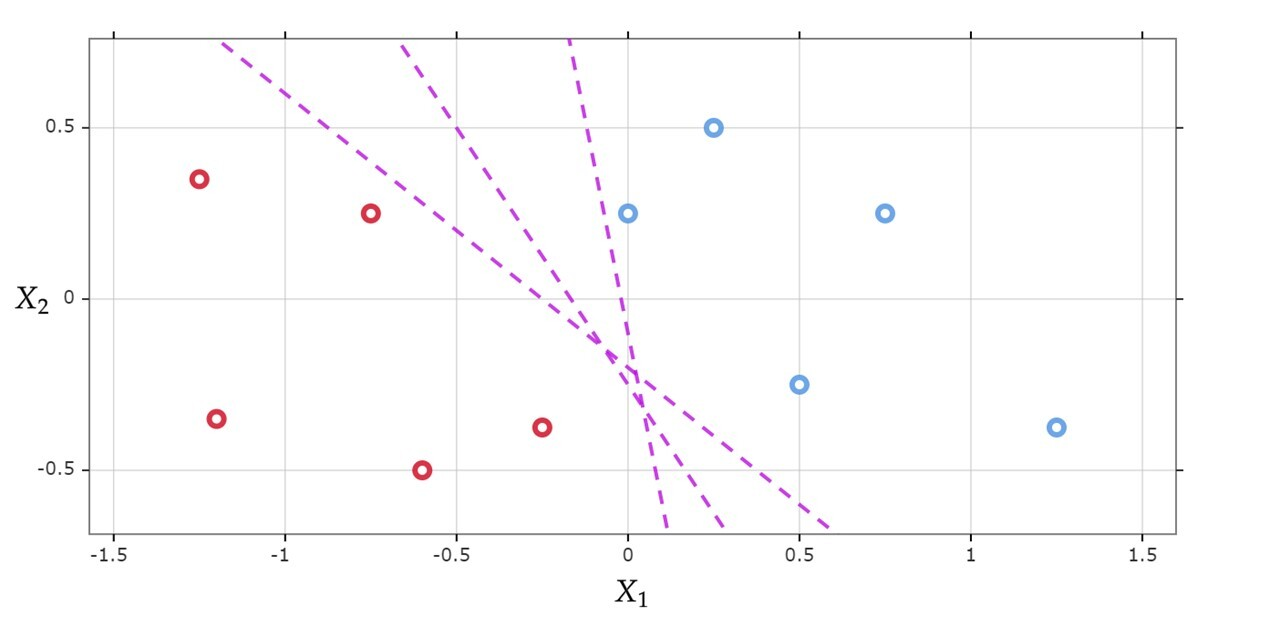
\includegraphics[width=\imgMed]{images/theory/separating_hyperplanes.jpg}
	\caption{Beispiele für \textit{separierende Hyperplanes}} 
	\label{fig:separating_hyperplanes}
\end{figure}
Der Abstand zwischen der \textit{separierenden Hyperplane} und den nächst gelegenen Traingsobjekten beider Labels
wird als \textit{Margin} bezeichnet. Die \textit{Hyperplane}, deren \textit{Margin} am größten ist,
wird daraus folgend auch \textit{Maximal Margin Hyperplane} genannt.
Die Traingsobjekte, die am nächsten zu der \textit{Hyperplane} liegen und damit auch den selben Abstand zu dieser haben,
werden als die Stützvektoren bezeichnet. Sie 'stützen' die \textit{Maximal Margin Hyperplane}.
Die Stützvektoren sind demnach die einzigen Traingsobjekte, die die Position der \textit{Hyperplane} überhaupt beeinflussen.\cite[S. 341]{james_2013}
Mit Hilfe der \textit{Maximal Margin Hyperplane} kann der 
\textit{Maximal Margin Classifier} nun neue unbekannte Testdaten klassifizieren, je nach dem auf welcher Seite sie liegen.
Je größer dabei die \textit{Margin} der zugrunde liegenden \textit{Hyperplane}, desto erfolgreicher der Klassifizierer.\cite[S. 1566]{noble_2006}

Eine solche \textit{Maximal Margin Hyperplane} ist in \ref{fig:maximal_margin} abgebildet. Die abbgebildeten Trainingsdaten sind die selben
wie auch in Abbildung \ref{fig:separating_hyperplanes}. Es wurde die 'mittigste' \textit{separierende Hyperplane} gefunden, die die Trainigsdaten
anhand ihrer Label trennen kann. Außerdem zu sehen, sind die am nächsten gelegen Trainigsobjekte auf beiden Seiten der \textit{Hyperplane}, die als
Stützvektoren dienen. Die \textit{Margin} wird visualisiert, durch die beiden Geraden, die parallel zur \textit{separierenden Hyperplane} liegen und
durch die beiden Stützvektoren verlaufen. Der Abstand dieser beiden Geraden zu der \textit{Hyperplane} ist die \textit{Margin}.
\begin{figure}[H]
	\centering
	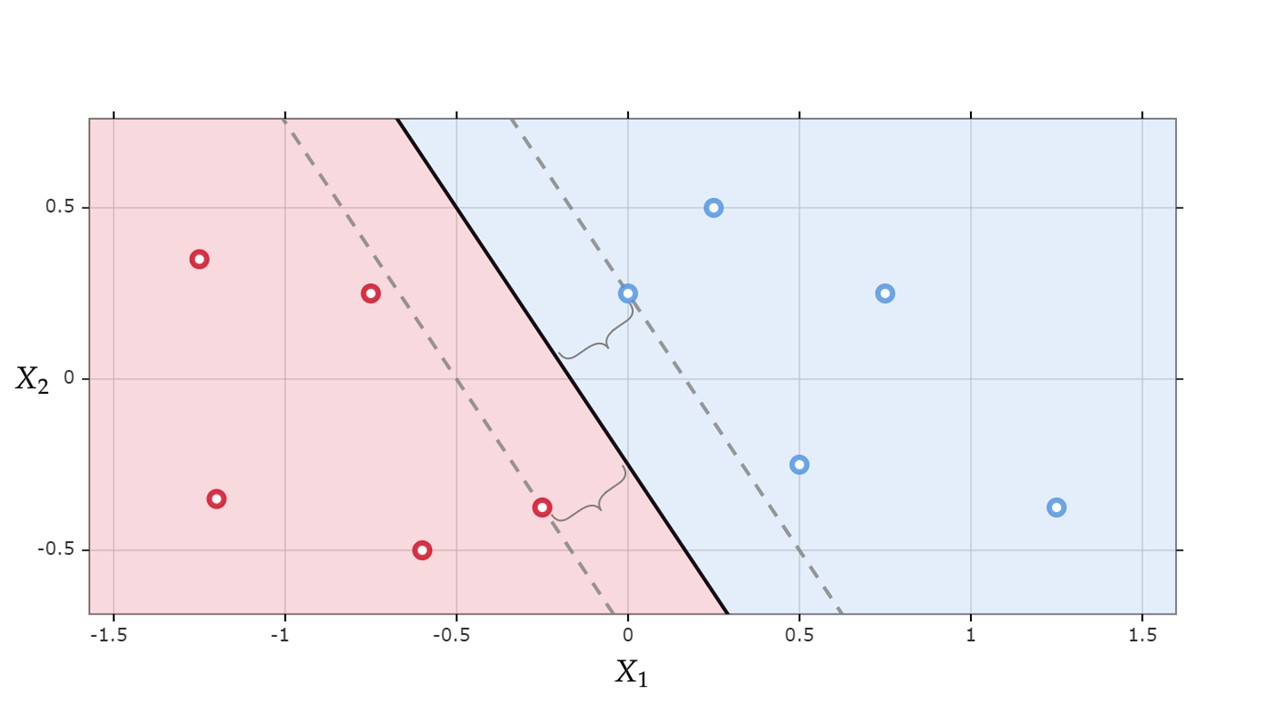
\includegraphics[width=\imgMed]{images/theory/maximal_margin.jpg}
	\caption{Beispiel für eine \textit{Maximal Margin Hyperplane}} 
	\label{fig:maximal_margin}
\end{figure}
Je nach Traingsdaten gibt es Szenarien in denen keine \textit{separierende Hyperplane} existiert, die die Daten perfekt anhand ihrer Label
trennen kann oder die \textit{Hyperplane} liegt nicht optimal um eine effiziente Klassifizierung durchführen zu können, da die
Stützvektoren ungünstig liegen. Der \textit{Maximal Margin Classifier} hat eine hohe Sensibilität für einzelne Trainingsobjekte
und kann demnach leicht übertrainiert werden. Es können zum Beispiel Trainigsobjekte existieren, deren \textit{Features} nicht den Normen einer Klasse entsprechen 
und damit eine Anomalie darstellen. Das besagte Trainigsobjekt würde dann auf der falschen Seite der zuvor gefundenen \textit{Hyperplane} liegen.
Deswegen müssen um eine bessere Klassifizierung und eine höhere Robustheit für einzelne Traingsobjekte
zu gewährleisten auch nicht perfekt \textit{separierende Hyperplanes} in Betracht gezogen werden.\cite[S. 343 - 345]{james_2013}

Dies wird vom \textit{Support Vector Classifier} umgesetzt. Er wird auch als \textit{Soft Margin Classifier} bezeichnet.
Wie der Name schon sagt, besitzt dieser eine 'weiche' \textit{Margin}. 
Der \textit{Support Vector Classifier} erweitert den bereits besprochenen \textit{Maximal Margin Classifier}
um eine eine 'weiche' \textit{Margin}, die von einem nutzerdefinierten Parameter abhängig ist.
Der Nutzer muss selbst entscheiden, wie durchlässig die \textit{Margin} sein soll und
wie vielen Traingsobjekten erlaubt werden soll die \textit{Margin} zu durchdringen ohne deren finale Ausrichtung zu beeinflussen.
Wie dieser Parameter gesetzt werden muss hängt von den Trainigsdaten und dem gewünschten Ergebnis ab
und muss durch Ausprobieren ermittelt werden.
Beim Setzen dieses Parameters muss zwischen Durchlässigkeit der \textit{Hyperplane} und der Breite der \textit{Margin} abgewägt werden.
Durch diese 'weiche' \textit{Margin} werden vereinzelt Testobjekte mit anormalen Charakteristiken der falschen Klasse
zugeordnet. Für die meisten Testobjekte steigt jedoch die Genauigkeit der Klassifizierung und aufgrund der 'weichen' \textit{Margin}
ist es leichter eine \textit{separierende Hyperplane} zu finden.\cite[S. 1566]{noble_2006}

Trotzdem gibt es immer noch Szenarien bei denen die Trainingsdaten nicht durch einen \textit{Support Vector Classifier} getrennt
werden können. In manchen Fällen sind die Trainingsdaten nicht linear zu trennen.
In diesen Fällen muss der \textit{Feature}-Raum erweitert werden. Hierfür wurde aus dem \textit{Support Vector Classifier}
die \textit{Support Vector Machine} entwickelt. Dabei wurden sogenannte \textit{Kernel}-Funktionen hinzugefügt.
Mit Hilfe von quadratischen, kubischen oder weiteren Polynomfunktionen höherer Grade wird der \textit{Feature}-Raum der
Traingsobjekte erweitert. Auf Basis der bisherigen \textit{Features} werden so mathematisch neue \textit{Features} berechnet, die 
dann womöglich durch eine \textit{Hyperplane} zu trennen sind, jedoch von den ursprünglichen \textit{Features} abhängig sind.
Der \textit{Feature}-Raum wird sogesehen von den \textit{Kernel}-Funktionen um eine oder mehrere Dimensionen erweitert.
Auch bei diesen \textit{Kernel}-Funktionen gibt es keine genaue Regel und die für für die Traingsdaten passende 
\textit{Kernel}-Funktion muss durch Ausprobieren gefunden werden. So können nun auch nichtlineare Daten klassifiziert werden.
\cite[S. 1566f.]{noble_2006}\cite[S. 224 - 227]{suthaharan_2015}

Die nachfolgende Abbildung \ref{fig:non_linear_data} zeigt zwei Beispiele hypothetischer Trainingsdaten, die nicht linear zu trennen sind.
Der \textit{Feature}-Raum wurde dann mit Hilfe einer \textit{Kernel}-Funktion erweitert und es konnte in einem höherdimensionalen Raum eine
\textit{separierende Hyperplane} gefunden werden, die die Trainigsobjekte anhand ihrer Labels trennen kann. 
Die zwei Grafiken zeigen nun wie diese höherdimensionale \textit{Hyperplane} in einem $2$-dimensionalen Raum aussehen würde 
und wie sie die Daten anhand ihrer Klasse aufteilt.
\begin{figure}[H]
	\centering
	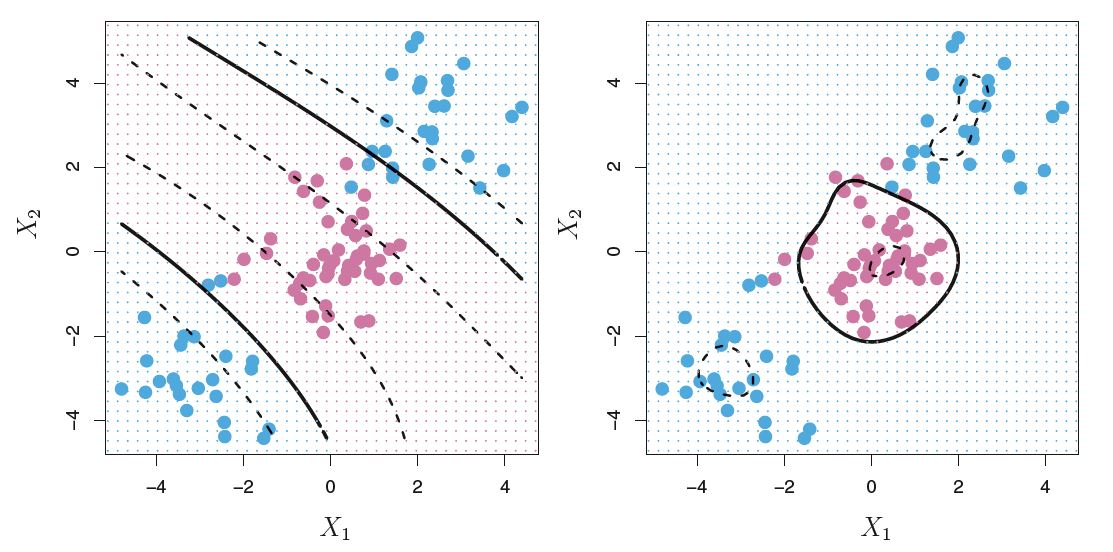
\includegraphics[width=\imgMed]{images/theory/non_linear_data.jpg}
	\caption{\textit{Hyperplanes} bei nichtlinearen Daten \cite[S. 353]{james_2013}} 
	\label{fig:non_linear_data}
\end{figure}
Mit Hilfe der \textit{Support Vector Machine} können wir nun einen Großteil an Datensätzen klassifizieren. 
Eine \textit{separierende Hyperplane} kann die Trainingsdaten jedoch immer nur in zwei Klassen einteilen. 
Wie können dann handgeschriebene Ziffern und Zahlen durch eine \textit{Support Vector Machine} erkannt werden?
Es gibt zwei Möglichkeiten dies zu bewerkstelligen, wenn $K > 2$ Klassen existieren.
Die erste Methode ist die 1-gegen-1-Klassifizierung. Hier wird für jede Paarung der Klassen $K \choose 2$
wird eine SVM erzeugt. Bei einer Klassifizierung eines neuen Testobjektes wird die Klasse ausgewählt, zu der das Objekt bei den
$K \choose 2$ paarweisen Klassifizierern am häufigsten zugewiesen wurde.
Die Alternative zu dieser Methode ist die 1-gegen-alle-Klassifizierung. Hier werden $K$ SVMs erstellt.
Eine SVM für jede Klasse und die $K-1$ restlichen Klassen. Ein unbekanntes Testobjekt wird dann der Klasse zugeordnet,
bei der die SVM sich am sichersten bei der Zuordnung ist. 
So kann die \textit{Support Vector Machine} auch Testobjekte verschiedener Klassen unterscheiden.\cite[S. 355f.]{james_2013}\cite[S.1567]{noble_2006}


\begin{minipage}{\textwidth}
	\begin{lstlisting}[language=Python, caption=Testcode, label=lst:beispielcode]
    from sklearn import svm
    svm_classifier = svm.SVC(gamma=0.001)
    svm_classifier.fit(X_train, y_train)
    predicted = svm_classifier.predict(X_test)
    _, axes = plt.subplots(2, 4)
    images_and_labels = list(zip(digits.images, digits.target))
    for ax, (image, label) in zip(axes[0, :], images_and_labels[:4]):
        ax.set_axis_off()
        ax.imshow(image, cmap=plt.cm.gray_r, interpolation='nearest')
        ax.set_title('Training: %i' % label)
        
    images_and_predictions = list(zip(digits.images[n_samples // 2:], predicted))
    for ax, (image, prediction) in zip(axes[1, :], images_and_predictions[:4]):
        ax.set_axis_off()
        ax.imshow(image, cmap=plt.cm.gray_r, interpolation='nearest')
        ax.set_title('Prediction: %i' % prediction)
    print("\nClassification report for classifier %s:\n%s\n" % (svm_classifier, metrics.classification_report(y_test, predicted)))
    disp = metrics.plot_confusion_matrix(svm_classifier, X_test, y_test)
    disp.figure_.suptitle("Confusion Matrix")
    print("\nConfusion matrix:\n%s" % disp.confusion_matrix)
    print("\nAccuracy of the Algorithm: ", svm_classifier.score(X_test, y_test))
    plt.show()
	\end{lstlisting}
\end{minipage}


\subsection{CNN}
Die Convolutional Neural Networks (CNN) sind vergleichbar zu den traditionellen Neuronalen
Netzwerken. Im Aufbau ähneln sie sich darin, dass beide Modelle aus Neuronen mit Gewichten 
bestehen, die ein Skalarprodukt aus einer Eingabe bilden. Das CNN besitzt ebenfalss eine
Verlustfunktion. Ein typisches Neuronales Netzwerk erhält als Eingabe einen einzigen Vektor und
wird in verscheidenen Schichten verarbeitet. 
Jede Schicht wird aus Gruppen von Neuronen gebildet, die jeweils mit den Neuronen aus der vorherigen
Schicht verknüpft sind. Die Neuronen, die sich in der selben Schicht befinden, teilen keine Verküpfungen und sind
unabhängig von den anderen.

Dabei existieren drei Hauptarten von Schichten in einem gewöhnlichen CNN, die Filter-Schichten (engl. Convolutional Layer), Aggregations-Schichten (Pooling Layer) 
und den vollständig verbundenen Schichten (engl. Fully Connected Layer, Dense Layer). 
Zusätzlich gibt es eine Eingabeschicht und eine Ausgabeschicht. Die Ausgabeschicht stellt dabei eine vollständig verknüpfte Schicht dar.

\subsubsection{Input Layer}
In der Eingabeschicht werden die Bilddaten gespeichert und in einer dreidimensionlae Matrix dargestellt.

\subsubsection{Filter-Schicht}
Die Filterschicht, auch häufig als Feature-Extraction-Layer bezeichnet, extrahiert Eigenschaften aus dem Eingabebild und übt die Hauptanzahl an Berechnungen aus. 
Es handelt sich hierbei um Faltungsoperationen, die Ähnlichekeiten zur Fourier-Transformation und zur Lapace-Transformation aufweisen, und bilden das Merkmal eines CNNs.
Ein Neuron einer Filterschicht betrachet ein bestimmten Bereich einer vorherigen Schicht in Form einer Matrix und bildet daraus ein Skalarprodukt, um die den Bereich auf nur eine Zahl zu reduzieren.
Die Architektur eines CNNs, die aus den verschiednenen Schichten und der Filter-Schichten besteht, ermöglichen, dass weniger Neuronen benötigt werden im Gegensatz zu anderen Mulitlayer Neuronalen Netzwerken.

\subsubsection{Aggregations-Schicht}


\subsection{Auswertung des Vergleiches}
